\documentclass[t]{beamer}

%\setbeameroption{show only notes}

\def\PresTitle{Bicycle Crashes in KY - 2013}
\font\footnoteFont=phvr7t at 8pt
\font\footnoteRefFont=phvro7t at 8pt
\font\thFont=phvb7t at 12pt
\newfont{\codeFont}{cmtt10 scaled 800}
\setbeamerfont{verbatim}{size={\fontsize{8pt}{10pt}}}
\mode<presentation>
{
  \usetheme{Warsaw}
  \setbeamercovered{transparent}
}


\usepackage[english]{babel}

\usepackage{times}
%\usepackage[T1]{fontenc}
\usepackage{graphicx}
\usepackage{hyperref}
\usepackage{listings}

\title[\PresTitle]{\PresTitle}

\author[Steve Roggenkamp] % (optional, use only with lots of authors)
{Steve Roggenkamp\\
}

\date[13 Nov 2015] % (optional)
{13 Nov 2015 \\
 }

\subject{\PresTitle}

\begin{document}

{%
\usebackgroundtemplate{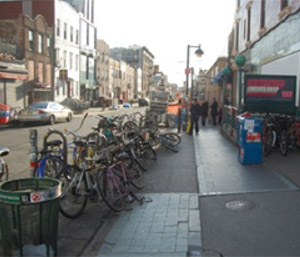
\includegraphics[height=\paperheight,width=\paperwidth]{bikesintown.jpg}}%
\begin{frame}
  \titlepage
  \setlength{\unitlength}{1cm}
\end{frame}
}%

\begin{frame}{Agenda}
  \begin{columns}
    \begin{column}[r]{6cm}
      \setlength{\unitlength}{1cm}
      \begin{picture}(0.0,0.0)(0.0,7.5)
        \includegraphics[scale=0.75]{pic1.jpg}
      \end{picture}
    \end{column}
    \begin{column}[l]{8cm}
      \begin{itemize}
      \item Problem definition
      \item Data sources and methods
      \item Data analysis
      \item Results
      \item Summary
      \item Q \& A
      \end{itemize}
    \end{column}
  \end{columns}
\end{frame}

{%
  \usebackgroundtemplate{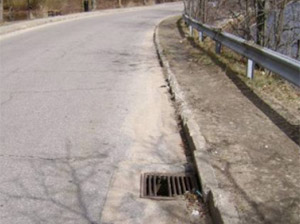
\includegraphics[height=\paperheight,width=\paperwidth]{grate.jpg}}%
\begin{frame}{Problem Definition}

  \begin{itemize}
  \item What can we learn from official collision extracts to be safer bicyclists?
  \end{itemize}
  \note{}
\end{frame}
}

\begin{frame}{Safety and risks - Crash stats}
  \begin{tabular}{llr}
    {\bf Fault\footnote{Statistics from League of American Bicyclists, Traffic Skills 101 manual}}&{\bf Action}&{\bf Pct}\\
    Bicyclist & Wrong way riding facing traffic & 14\% \\
    Bicyclist & Left turn from the right side of the road & 11\% \\
    Bicyclist & Failure to yield from driveway & 9\% \\
    Bicyclist & Running a stop sign or signal & 8\% \\
    Bicyclist & Swerving in front of car & 5\% \\
    {\bf Bicyclist}&{\bf Total}&{\bf 47\%}\\
    Motorist  & Left turn in front of the bicyclist & 13\% \\
    Motorist  & Right turn in front of bicyclist & 11\% \\
    Motorist&Running stop sign or signal& 8\%\\
    Motorist  & Opening car door into path of the bicyclist & 7\% \\
    Motorist  &Failure to yield from driveway& 6\%\\
    Motorist&Didn't see the cyclist& 3\%\\
    {\bf Motorist}&{\bf Total}&{\bf 48\%}\\
    Unknown & & 5\% \\
  \end{tabular}
\end{frame}

\begin{frame}{Traffic safety statistics}
  More crash statistics\footnote{From NHTSA Traffic Safety Facts, 2010}
  \begin{itemize}
    \item Kentucky had 7 bicyclist deaths in 2010
    \item Kentucky's fatality per million population, 1.61, is below national average, 2.00
    \item Male fatality rate, 3.51, is about 7x higher than female, 0.53
    \item Male injury rate, 256, is about 3x higher than female, 81
    \item Alcohol is involed in a significant percentage of crashes, 30-34%
  \end{itemize}
\end{frame}

\begin{frame}{Data sources and methods}
  \begin{itemize}
  \item \href{http://crashinformationky.org/KCAP/Public/Home.aspx}{Kentucky State Police Collision Extract web site}
    \begin{itemize}
      \item Used data from 2013
      \item Data from 2010-2014 are available from site
    \end{itemize}
  \item \href{http://virtuoso.openlinksw.com/}{Virtuoso Universal Server}
    \begin{itemize}
      \item Linked data storage
      \item SPARQL endpoint
      \item Ubuntu 14.04LTS version 06.01.3127
    \end{itemize}
  \item \href{http://r-project.org}{R Project for Statistical Computing}
    \begin{itemize}
      \item Statistical analysis
      \item Data visualization
      \item version 3.2.2 (Fire Safety)
    \end{itemize}
  \item Custom software
    \begin{itemize}
      \item Perl code to transform dumped data to RDF triples (TURTLE)
      \item SPARQL queries embedded in R code
    \end{itemize}
  \end{itemize}
  \note{}
\end{frame}

%% \begin{frame}{FRAME TITLE}
%%   \begin{block}{Normal Block}
%% Some blocky text   
%%   \end{block}
%%   \begin{alertblock}{Alert Block}
%% Some alerty text   
%%   \end{alertblock}
%%   \begin{exampleblock}{Example Block}
%% Some example text   
%%   \end{exampleblock}
%%   \begin{block}{Normal Block}
%% Normal outer block
%%   \begin{exampleblock}{Example Block}
%% Example block within Normal block
%%   \end{exampleblock}
%%   \end{block}
%%   \note{}
%% \end{frame}
%% 

\begin{frame}{Collision Data Relationships}
  \begin{figure}
    \includegraphics[scale=0.6]{ExtractDataRelations.png}
  \end{figure}
\end{frame}

\setbeamerfont{codeFont}{size=\scriptsize}

\begin{frame}[fragile]{Initial explorations - number of RDF triples}
\usebeamerfont{codeFont}
  \begin{block}{nTriples.R}
    \begin{verbatim}
library(httr)
library(readr)
sparqlEndpoint <- "http://localhost:8890/sparql/"
sparqlQuery    <- "select (count(*) as ?nTriples) \
  from <http://steveroggenkamp.com/kycrashdata/> \
  where \{ ?s ?p ?o \}" 
out <- POST( sparqlEndpoint, 
             encode="multipart",
             body=list( query=sparqlQuery),
             add_headers( Accept="text/csv; charset=UTF-8" ))
data <- read_csv(rawToChar(out$content))
    \end{verbatim}
 \end{block}
 \begin{block}{R environment}
   \begin{verbatim}
> source("nTriples.R")
> data\$nTriples
[1] 7087530
> 
  \end{verbatim}
  \end{block}
\end{frame}

\begin{frame}{FRAME TITLE}
  \begin{itemize}
  \item 
    \begin{itemize}
      \item 
      \item 
      \item 
    \end{itemize}
  \item 
  \item 
  \item 
  \end{itemize}
  \note{}
\end{frame}

\begin{frame}{FRAME TITLE}
  \begin{itemize}
  \item 
    \begin{itemize}
      \item 
      \item 
      \item 
    \end{itemize}
  \item 
  \item 
  \item 
  \end{itemize}
  \note{}
\end{frame}


\end{document}
